% Created 2020-01-20 Пн 22:07
% Intended LaTeX compiler: pdflatex
\documentclass[presentation]{beamer}
\usepackage[utf8x]{inputenc}
\usepackage[T2A]{fontenc}
\usepackage{graphicx}
\usepackage{longtable}
\usepackage{wrapfig}
\usepackage{rotating}
\usepackage[normalem]{ulem}
\usepackage{amsmath}
\usepackage{textcomp}
\usepackage{amssymb}
\usepackage{capt-of}
\usepackage{minted}
\usepackage{hyperref}
\usepackage[condensed,math]{iwona}
\usepackage{fontspec}
\setmainfont[Ligatures=TeX]{Iwona Cond}
\usepackage{polyglossia}
\setmainlanguage{english}
\setotherlanguage{russian}
\setminted{fontsize=\footnotesize}
\usetheme{Luebeck}
\author{Pavel}
\date{}
\title{Методы аунтетификации OAuth + UMA Protocol flow}
\hypersetup{
 pdfauthor={Pavel},
 pdftitle={Методы аунтетификации OAuth + UMA Protocol flow},
 pdfkeywords={},
 pdfsubject={},
 pdfcreator={Emacs 26.3 (Org mode 9.3)},
 pdflang={English}}
\begin{document}

\maketitle
\begin{frame}{Outline}
\tableofcontents
\end{frame}


\section{Теория: Авторизация}
\label{sec:org36890f9}

\begin{frame}[label={sec:orgf28ee89}]{OAuth 2.0}
\begin{center}
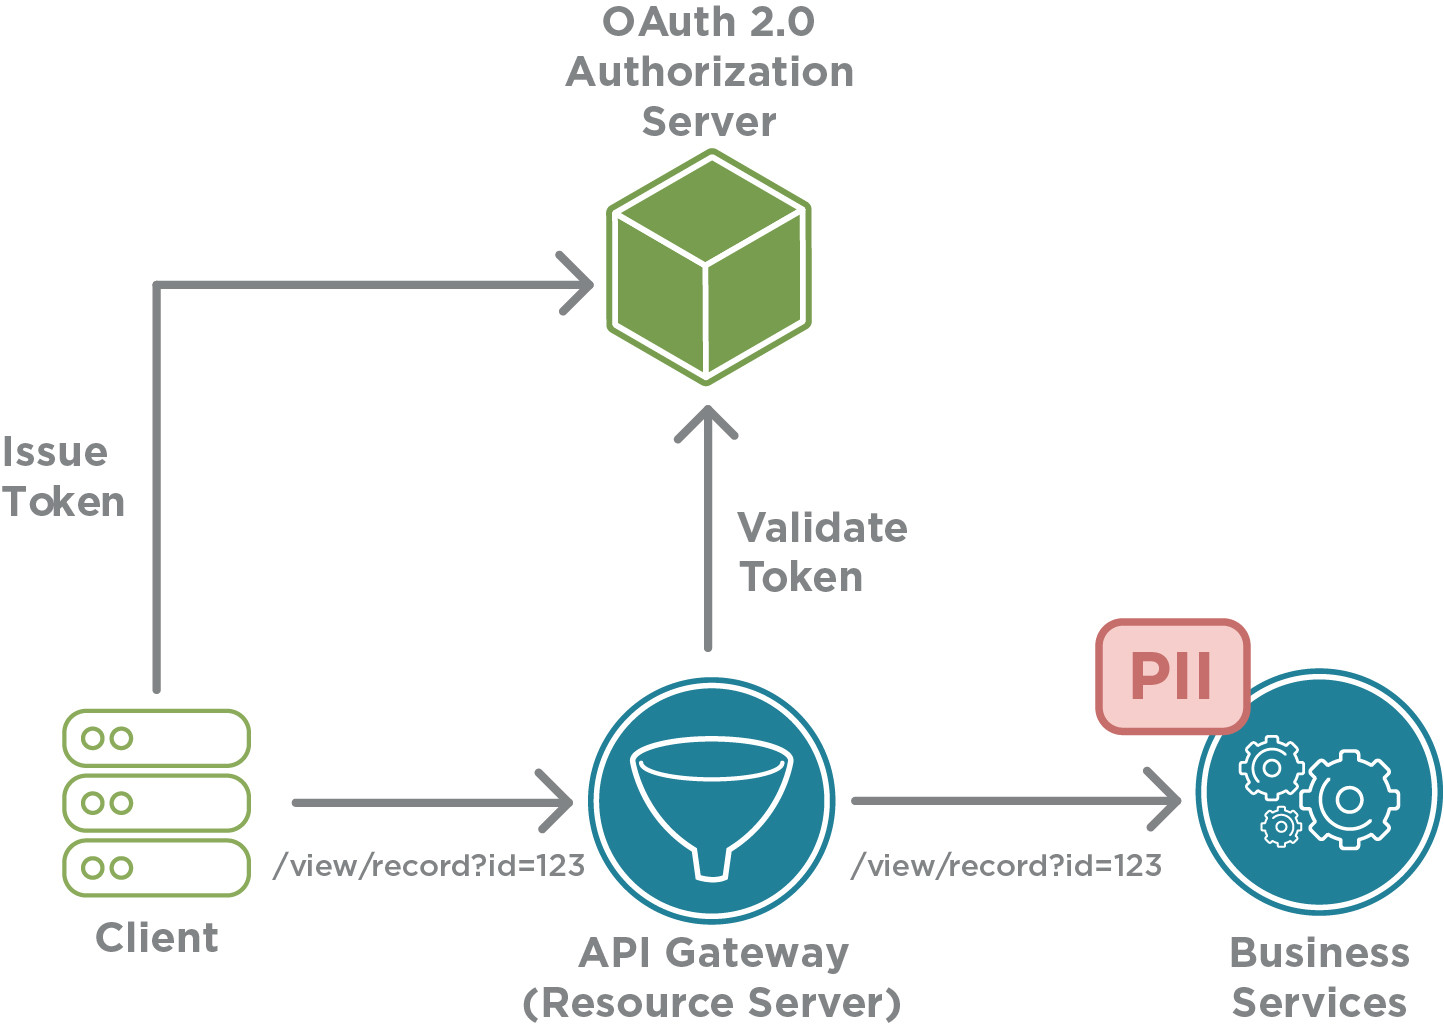
\includegraphics[width=0.7\textwidth]{./img/oauth2.jpg}
\end{center}
\end{frame}

\begin{frame}[label={sec:org509c52e}]{OAuth 2.0}
\begin{enumerate}
\item Client посылает запрос к Authorization Server (AS)
\item Если Client не залогинен (кука нет или не валидный)
\begin{enumerate}
\item AS выдает форму логина и проверяет, что пользователь вошел правильно.
Источник пользователей - откуда угодно (DB, LDAP, etc)
\end{enumerate}
\item AS возвращает некоторый Token
\item API Gateway видит запрос с Token
\item API Gateway отправляет Token на AS
\item Если Token верный, AS одобряет.
\end{enumerate}


Доступ к отдельным объектам (Entities) в такой модели регулируется протоколом UMA
\end{frame}

\begin{frame}[label={sec:orga6e4dcc}]{OAuth 2.0 + UMA}
\begin{center}
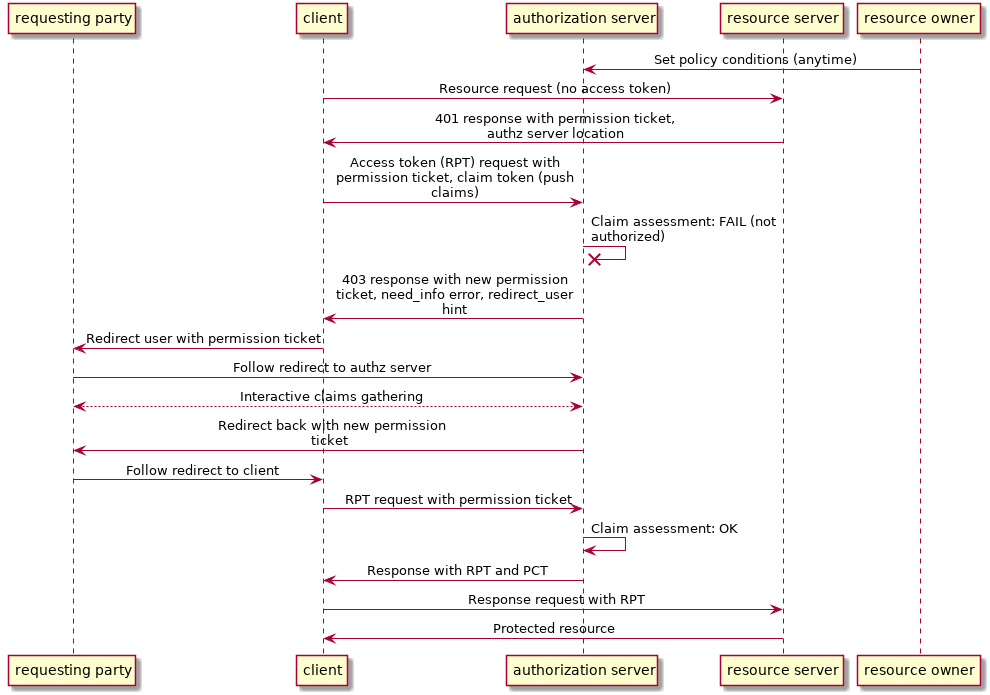
\includegraphics[width=.9\linewidth]{img/uma.png}
\end{center}
\begin{center}
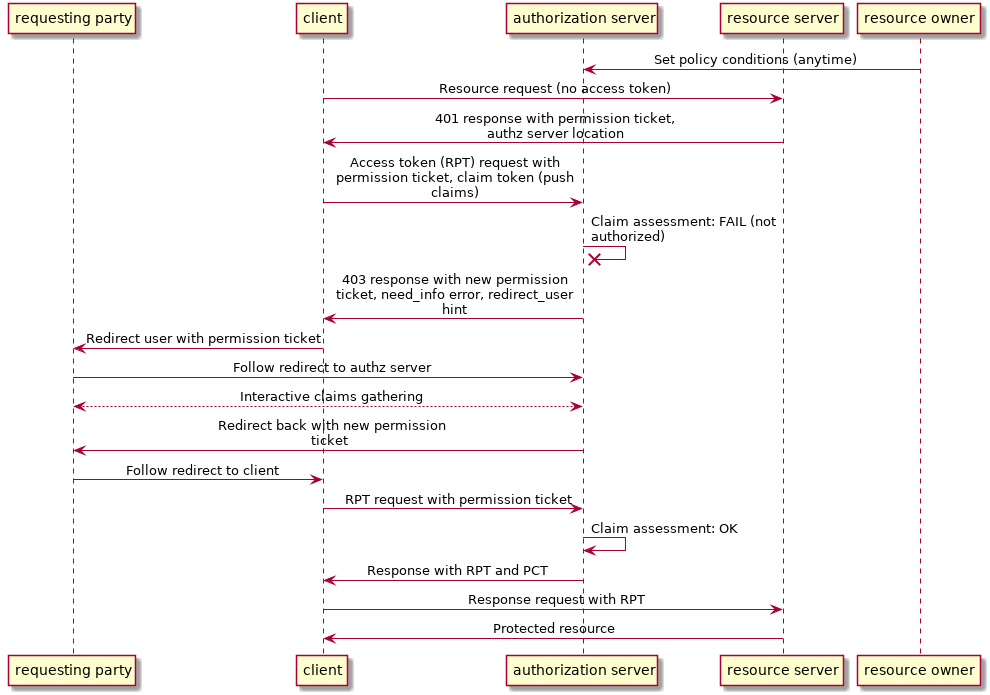
\includegraphics[width=0.7\textwidth]{img/uma.png}
\end{center}

\begin{block}{Определения на схеме:}
\begin{itemize}
\item Requesting party - браузер
\item client - клиент, который хочет получить доступ к определенному ресурсу (часть веб-приложения или сам requesting party)
\item RPT - requesting party token - токен доступа OAuth
\item permission - авторизация доступа к определенному ресурсу с некоторому набором прав (scopes), привязанных к ресурсу
\item permission ticket - handle, представляющий запрошенные права доступа (permissions), необходимый в запросах к серверу авторизации
\item claim - запрос, представляющий требуемые атрибуты запрашиваемого ресурса/ов.
\item persisted claims token - токен, позволяющий много раз использовать набор claims для авторизации.
\end{itemize}
\end{block}
\end{frame}


\section{Теория: Примеры моделей контроля доступа}
\label{sec:org6301f42}
\begin{frame}[label={sec:org71be13d}]{DAC (Discretionary Access Control)}
\begin{itemize}
\item модель контроля доступа, который может быть передан субъектом другим субъектам. Например, \uline{владелец} файлов в UNIX может передать права на файлы другим субъектам.
\end{itemize}
\end{frame}

\begin{frame}[label={sec:org50bb317}]{MAC (Mandatory Access Control)}
\begin{itemize}
\item модель контроля доступа, в которой реализация запрещает субъектам передавать права доступа. Права доступа определяются администратором системы.
\end{itemize}
\end{frame}



\begin{frame}[label={sec:org2867552}]{RBAC (Role-Based Access Control)}
\begin{center}
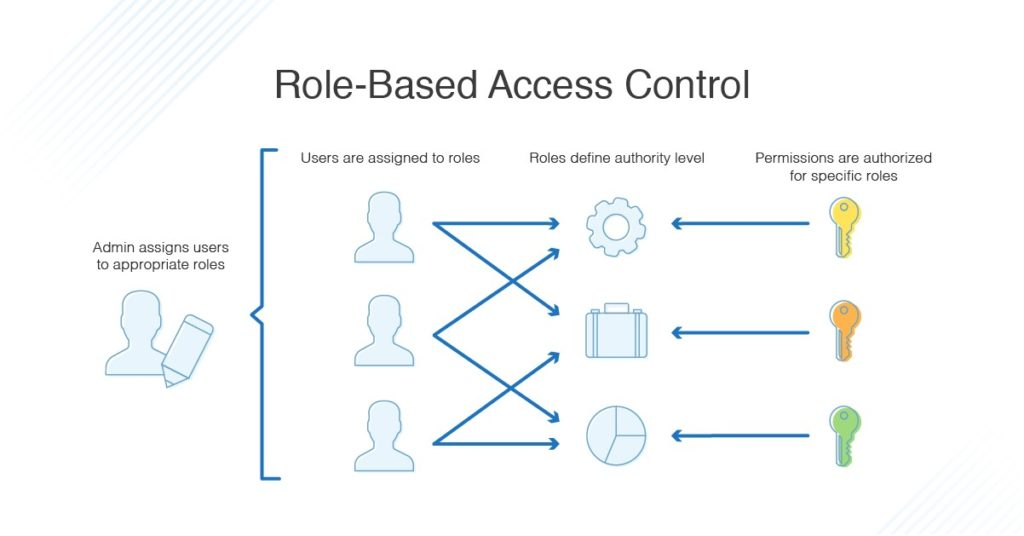
\includegraphics[width=0.6\textwidth]{./img/rbac.jpg}
\end{center}

\begin{itemize}
\item Модель контроля доступа, в которой доступ к операции  производится на основании того, содержит ли роль субъекта соответствующую привилегию.

\item Роль - множество привилегий, доступных пользователям

\item Субъекту может быть присвоено несколько (0\ldots{}n) ролей. Роли может быть присвоено несколько привилегий.
\end{itemize}
\end{frame}



\begin{frame}[label={sec:orgcf7b9c8}]{ABAC (Attribute-Based Access Control)}
во внимание принимаются свойства (атрибуты) субъекта или объекта, а также свойства окружения (дата, время доступа).

\begin{center}
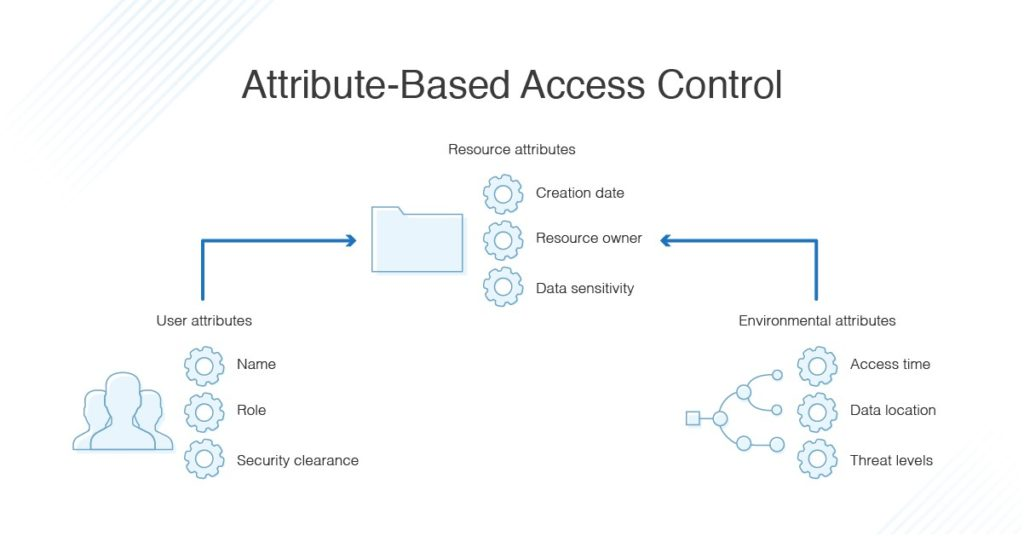
\includegraphics[width=0.5\textwidth]{./img/abac.jpg}
\end{center}
Например:
\begin{itemize}
\item Пользователь(sub) может просмотреть документ(obj), если он(obj) создан коллегами из того же департамента
\item Пользователь(sub) может редактировать документ(obj), если он(subj) создал его(obj) и установлен режим черновика(obj).
\end{itemize}
\end{frame}

\section{Рассмотренные решения}
\label{sec:org0e9d8e4}

\begin{frame}[label={sec:orga120c36}]{Shiro}
\begin{itemize}
\item Сайт: \url{https://shiro.apache.org}
\item Java, лицензия Apache2
\item OAuth2 поддерживается отдельным решением: \url{https://github.com/bujiio/buji-pac4j}
\item Источник данных о пользователях - любой: для этого надо реализовать интерфейс \href{https://shiro.apache.org/realm.html}{Realm}.
\item Хорошая документация
\item RBAC и item-based permissions (механизм авторизации - любой, прописывается в Java-коде)
\end{itemize}
\end{frame}
\begin{frame}[label={sec:org7f5fa22}]{Shiro: Механизм аутентификации}
\alert{Subject} - принятый термин для пользователя

\begin{center}
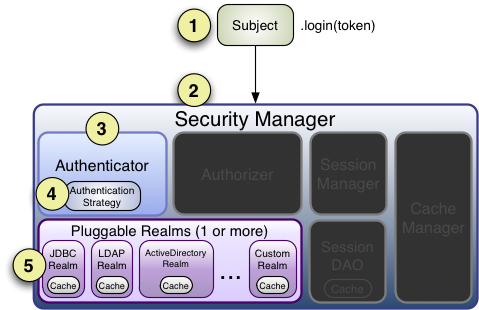
\includegraphics[width=.9\linewidth]{./img/ShiroAuthenticationSequence.png}
\end{center}
\end{frame}

\begin{frame}[label={sec:org6038756},fragile]{Shiro: Механизм аутентификации}
 \begin{enumerate}
\item Приложение вызывает \texttt{Subject.login} с аргументом типа \texttt{AuthenticationToken} (\texttt{token})
\item экземпляр \texttt{Subject} вызывает \texttt{SecurityManager.login} с этим аргументом
\item \texttt{SecurityManager} вызывает \texttt{Authenticator.authenticate(token)}
\item \texttt{Authenticator} выбирает \texttt{Realm} (источник данных о пользователе) и вызывает его, используя сконфигурированную \texttt{AuthenticationStrategy}.
\item Каждый из доступных \texttt{Realm}'ов сообщает, поддерживает ли он \texttt{token} данного типа, и если да, то для него вызывается \texttt{getAuthenticationInfo(token)}, в котором производится попытка аунтетификации.
\end{enumerate}
\end{frame}

\begin{frame}[label={sec:org44023ca},fragile]{Shiro: Механизм авторизации}
 \begin{block}{AuthenticationStrategy}
Определяет, нужно ли аунтетифицировать по всем Realm или только по одному до первой успешной аунтетификации, и так далее.
\end{block}

\begin{block}{Механизм авторизации}
Когда вызывается метод \texttt{Subject.isPermitted()} или \texttt{Subject.checkPermission()}

\begin{enumerate}
\item \texttt{Subject} делегирует в \texttt{SecurityManager}
\item \texttt{SecurityManager} делегирует в \texttt{Authorizer}
\item \texttt{Authorizer} опрашивает \texttt{Realm}'ы:
a. \texttt{Realm} Получает все Permissions и аггрегирует результат, затем делает wildcard matching.
\end{enumerate}
\end{block}
\end{frame}



\begin{frame}[label={sec:org9649da7}]{Shiro: минусы}
\begin{itemize}
\item Отлично подходит для авторизации доступа, но нет возможности программно получить  все объекты, к которым пользователь имеет доступ
\item В списке рассылки предложили организовать получение всех объектов через свою базу данных (свой интерфейс Realm) - поэтому это решение было отклонено
\item Нет поддержки OAuth2 из коробки
\end{itemize}
\end{frame}

\begin{frame}[label={sec:orge4f4200},fragile]{Keycloak}
 \begin{itemize}
\item "Коробочное решение" для авторизации с интерфейсом админа,  поддерживаемое RedHat
\item Правила доступа интегрируются в Spring Boot "из коробки" с несколькими строчками конфига \texttt{application.properties}
\item Правила доступа задаются в графическом интерфейсе или с помощью JavaScript - с использованием следующих параметров:
\begin{enumerate}
\item Время доступа
\item Членство в роли (RBAC)
\item Email пользователя и многие другие атрибуты:
\end{enumerate}
\end{itemize}
\begin{minted}[]{js}
var context = $evaluation.getContext();
var identity = context.getIdentity();
var attributes = identity.getAttributes();
var email = attributes.getValue('email').asString(0);
if (identity.hasRealmRole('admin') || email.endsWith('@keycloak.org')) {
    $evaluation.grant();
}
\end{minted}
\end{frame}

\begin{frame}[label={sec:org6d5a3e8},fragile]{Keycloak: продолжение}
 \begin{itemize}
\item Права доступа могут задаваться на отдельный ресурс или на "scope" - действие над группой ресурсов (например \texttt{="book:read"=}), или на группу ресурсов, объединенную общим типом (например \texttt{="book"=})
\item Есть официальное Java API, будет использовано в Demo-приложении
\item Совместим с OAuth2/UMA
\item Можно получить список всех доступных пользователю permissions:
\end{itemize}
\begin{minted}[]{java}
var ar = new AuthorizationRequest();

   var response = getAuthzClient().authorization().authorize(ar);
   var rpt = getAuthzClient().protection().introspectRequestingPartyToken(response.getToken());
   for (Permission granted : rpt.getPermissions()) {
       System.out.println(granted.toString());
   }

\end{minted}
\end{frame}





\begin{frame}[label={sec:org1e8935c}]{ORY/Ladon}
\begin{itemize}
\item Golang
\item Совместим с OAuth2/UMA
\item Источник данных: Любая БД (необходимо реализовать один интерфейс для доступа, есть реализация для Redis)
\item \url{https://github.com/ory/ladon} лицензия Apache2.
\end{itemize}

\begin{block}{Возможно, стоит расмотреть его.}
\end{block}
\end{frame}

\section{Demo-решение на Java c использованием Spring Boot и  Keycloak}
\label{sec:org3811f7d}
\begin{frame}[label={sec:org0ee5f39}]{Архитектура}
\begin{itemize}
\item Приложение написано на Java и имеет JDBC-совместимый источник данных. Информация о правах доступа не хранится в базе данных, но каждой строке ставится в соответствие идентификатор из базы данных \alert{Keycloak}

\item Необходимо придумать, как конвертировать список permissions в ID базы данных, поскольку некоторые permissions могут предоставлять доступ не просто к отдельным ресурсам, но и по widlcard.

\item В данном приложении для этого используется сочетание UMA Permissions (DAC) и RBAC (библиотекарь/пользователь)
\begin{itemize}
\item У пользователя производится фильтрация по ID.
\end{itemize}
\end{itemize}
\end{frame}



\begin{frame}[label={sec:orgc247a04}]{Архитектура: взаимодействие}
\begin{center}
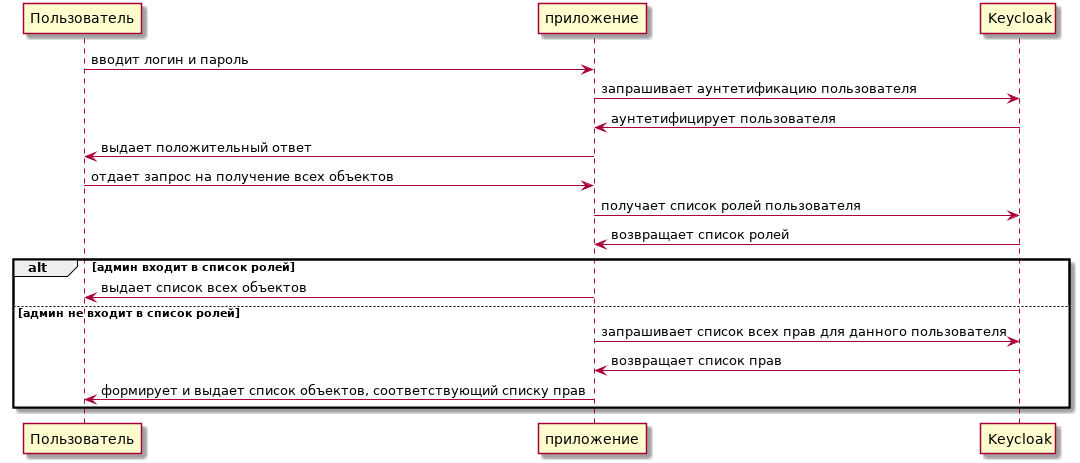
\includegraphics[width=.9\linewidth]{img/arch.png}
\end{center}
\end{frame}

\begin{frame}[label={sec:orga53298f}]{Подводные камни при реализации}
\begin{itemize}
\item Существует два API Keycloak permissions.
\begin{enumerate}
\item Permissions, редактируемые админом, могут быть простыми DAC/RBAC или сложными JavaScript
\item User-managed Access - permissions, которые могут быть заданы пользователем для других пользователей над ресурсами, которыми он владеет (это отключаемо, только DAC)
\end{enumerate}
\end{itemize}
\end{frame}


\begin{frame}[label={sec:org5cdfac3}]{Исходный код приложения}
\url{https://github.com/pashazz/library}
\end{frame}
\end{document}